% Biohub Cell Lineage Tracker — IEEE-style manuscript
% Compile: cd paper && pdflatex main && bibtex main && pdflatex main && pdflatex main
%
% Manual screenshot placeholders:
%   figures/ui_screenshot.png  — capture from: streamlit run app.py
% Other figures generated by: python scripts/generate_figures.py

\documentclass[journal]{IEEEtran}

\usepackage{cite}
\usepackage{amsmath,amssymb}
\usepackage{algorithmic}
\usepackage{graphicx}
\usepackage{textcomp}
\usepackage{xcolor}
\usepackage{hyperref}
\usepackage{booktabs}

\begin{document}

\title{Biohub Cell Lineage Tracker: An Open Pipeline and Interactive System for 3D Cell Tracking During Development}

\author{Tobi-Joshua Samuel}

\maketitle

\begin{abstract}
Three-dimensional time-lapse microscopy is a central tool for studying cell behavior during embryonic development.
Recovering accurate cell positions and lineage relationships from fluorescence volumes remains difficult because cells move, divide, overlap, and vary in intensity.
We present Biohub Cell Lineage Tracker, an open-source pipeline and interactive analysis application for detecting cells in 3D frames, linking them across time, and reconstructing lineage graphs with division events.
The system combines anisotropy-aware classical peak detection, Hungarian assignment with multi-cue linking costs, and conservative mitosis inference.
A Streamlit interface enables inspection of raw volumes, detection overlays, track structure, and exportable graph tables.
We describe the data model, algorithmic design, software architecture, and qualitative behavior on synthetic and zebrafish-style microscopy volumes.
The implementation is modular and extensible to learned detectors.
\end{abstract}

\begin{IEEEkeywords}
Cell tracking, lineage reconstruction, light-sheet microscopy, 3D image analysis, interactive visualization
\end{IEEEkeywords}

\section{Introduction}
Live imaging of developing organisms produces four-dimensional datasets that encode cell positions and ancestry.
Manual lineage tracing is accurate but slow and difficult to reproduce at scale.
Automated methods must therefore address detection in anisotropic 3D volumes, data association across time, and inference of cell division topology.

This work packages a reproducible analysis stack and a browser-based inspection tool for researchers who need to process volumes, review intermediate outputs, and export lineage graphs without modifying low-level code.
The design prioritizes interpretability, modularity, and publication-ready visualization over opaque end-to-end learning.

\section{Related Work}
Cell tracking in microscopy has been studied extensively.
TrackMate provides an extensible particle-tracking workflow within ImageJ/Fiji \cite{tinevez2017trackmate}.
Lineage reconstruction methods such as the approach of Amat \textit{et al.} emphasize linking in large live-imaging datasets \cite{amat2014lineage}.
Deep learning segmentation tools including Cellpose \cite{stringer2021cellpose} and 3D U-Net \cite{cicek20163dunet} improve detection quality when training data are available.
Classical peak detection and assignment remain strong baselines when annotations are sparse and runtime must stay predictable \cite{van2014scikit,kuhn1955hungarian}.

Interactive scientific tools lower the barrier to exploratory analysis.
Streamlit supports rapid construction of data-centric web interfaces \cite{streamlit2019}.
Our system combines a documented batch pipeline with such an interface for inspection and export.

\section{Dataset and Problem Formulation}
\subsection{Image data}
Each recording is a sequence $I_t(z,y,x)$, $t=0,\ldots,T-1$, where $t$ indexes time and $(z,y,x)$ are voxel coordinates.
Volumes are stored as compressed Zarr chunks with shape $(T,Z,Y,X)$ and uint16 intensities.
Physical voxel spacing is anisotropic:
$s_z = 1.625\,\mu\text{m}$ and $s_y=s_x=0.40625\,\mu\text{m}$.

\subsection{Lineage graph}
The target output is a directed graph $G=(V,E)$.
Each node $v\in V$ is a detection with attributes $(t_v,z_v,y_v,x_v)$.
Each edge $(u,v)\in E$ links a cell at time $t_u$ to its continuation or daughter at a later time.
A division is represented by one parent with two or more outgoing edges.

Training annotations, when available, are stored as GEFF graph directories with sparse centroid labels.
A missing label does not imply absence of a cell.

\section{Methods}
\subsection{Detection}
We preserve full axial resolution and average-pool lateral dimensions by a factor of four, yielding an approximately isotropic working grid.
A Gaussian-smoothed volume is thresholded using the maximum of Otsu's method and a relative-rise rule.
Local intensity maxima become centroid candidates \cite{van2014scikit}.
A secondary dense-cluster pass with smaller minimum peak spacing recovers nearby cells.
Centroids are refined by intensity-weighted averaging in a local neighborhood and filtered by physical non-maximum suppression.

\subsection{Temporal linking}
Consecutive frames are associated by solving a linear assignment problem \cite{kuhn1955hungarian} on a cost matrix
\begin{equation}
C_{ij} = d_{ij} + \lambda_m \rho^m_{ij} + \lambda_I f_{ij} + \lambda_N g_{ij},
\end{equation}
where $d_{ij}$ is physical Euclidean distance, $\rho^m_{ij}$ is motion residual from the previous displacement, $f_{ij}$ is normalized intensity difference, and $g_{ij}$ compares local neighborhood offset signatures.
Links above a distance gate are forbidden.

\subsection{Division inference}
After one-to-one assignment, unmatched detections may be linked as second daughters when a parent already has one child, sister distance is small, and the parent lies near the daughter midpoint.
This rule increases recall of mitosis events while limiting arbitrary fan-out.

\subsection{Post-processing}
Isolated detections that do not participate in any edge can be removed to reduce spurious nodes in exported graphs.

\section{System Architecture}
The repository is organized into reusable Python modules and a Streamlit front end:
\begin{itemize}
  \item \texttt{src/biohub/}: configuration, I/O, detection, tracking, analysis, export, and visualization;
  \item \texttt{app.py}: interactive application;
  \item \texttt{scripts/generate\_figures.py}: batch figure generation for manuscripts;
  \item \texttt{paper/}: \LaTeX{} source.
\end{itemize}
Figure~\ref{fig:pipeline} summarizes the processing flow.

\begin{figure}[!t]
  \centering
  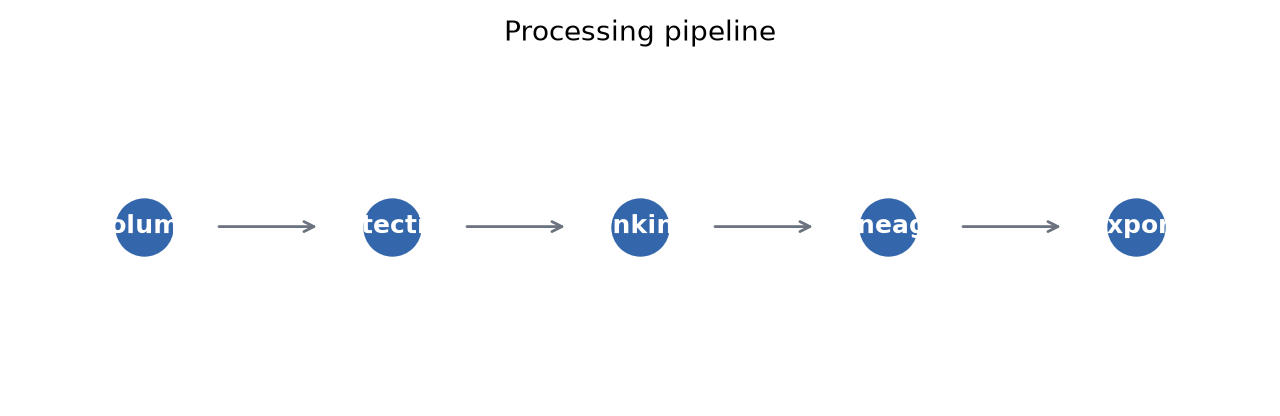
\includegraphics[width=\linewidth]{../figures/pipeline_overview.png}
  \caption{Processing pipeline from 3D time-lapse volume to exported lineage graph.}
  \label{fig:pipeline}
\end{figure}

\section{Implementation Details}
The pipeline streams one timepoint at a time to limit memory use.
Zarr chunks are decompressed with Blosc2.
Graph exports include CSV tables with separate node and edge rows and JSON graph documents for visualization.
A \texttt{LearnedDetector} interface is provided for future integration of pretrained segmenters without changing the tracking layer.

\section{Interactive Application}
The Streamlit application exposes seven views: overview, dataset summary, volume inspection, pipeline execution, detection overlay, lineage graph, and export.
Users may load a bundled synthetic sample, upload a NumPy array of shape $(T,Z,Y,X)$, or point to a local Zarr directory.
Sliders select time and $z$ indices; histograms summarize intensity; overlays show centroids and division markers.
Exports are available as CSV and JSON downloads.

\begin{figure}[!t]
  \centering
  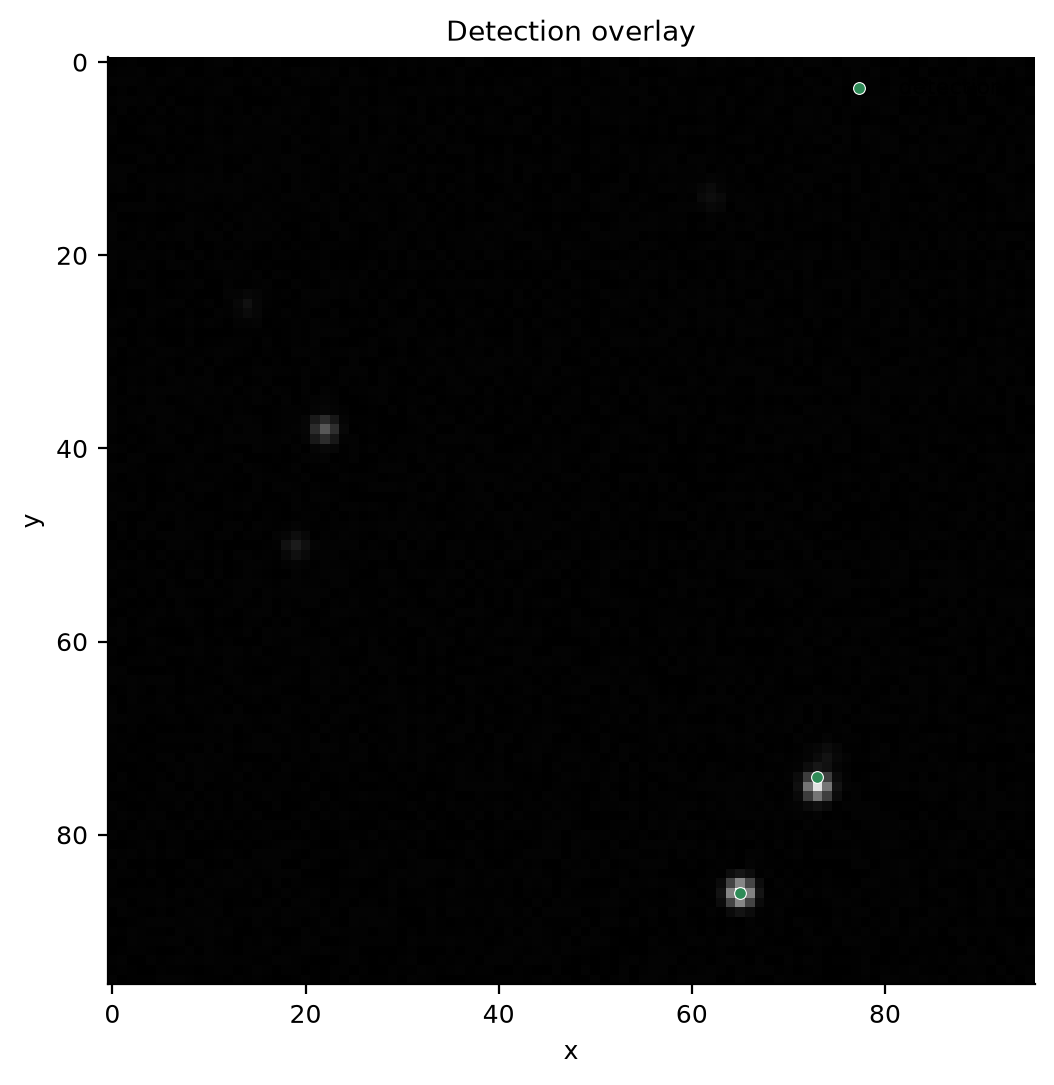
\includegraphics[width=\linewidth]{../figures/detection_overlay.png}
  \caption{Detection overlay on a representative $xy$ slice. Green markers indicate centroids.}
  \label{fig:detection}
\end{figure}

% --- Manual screenshot placeholder ---
% Capture the Streamlit home or Pipeline tab after running: streamlit run app.py
% Save as figures/ui_screenshot.png and uncomment the figure below.
%
% \begin{figure}[!t]
%   \centering
%   \includegraphics[width=\linewidth]{../figures/ui_screenshot.png}
%   \caption{Streamlit user interface for volume inspection and pipeline execution.}
%   \label{fig:ui}
% \end{figure}

\begin{figure}[!t]
  \centering
  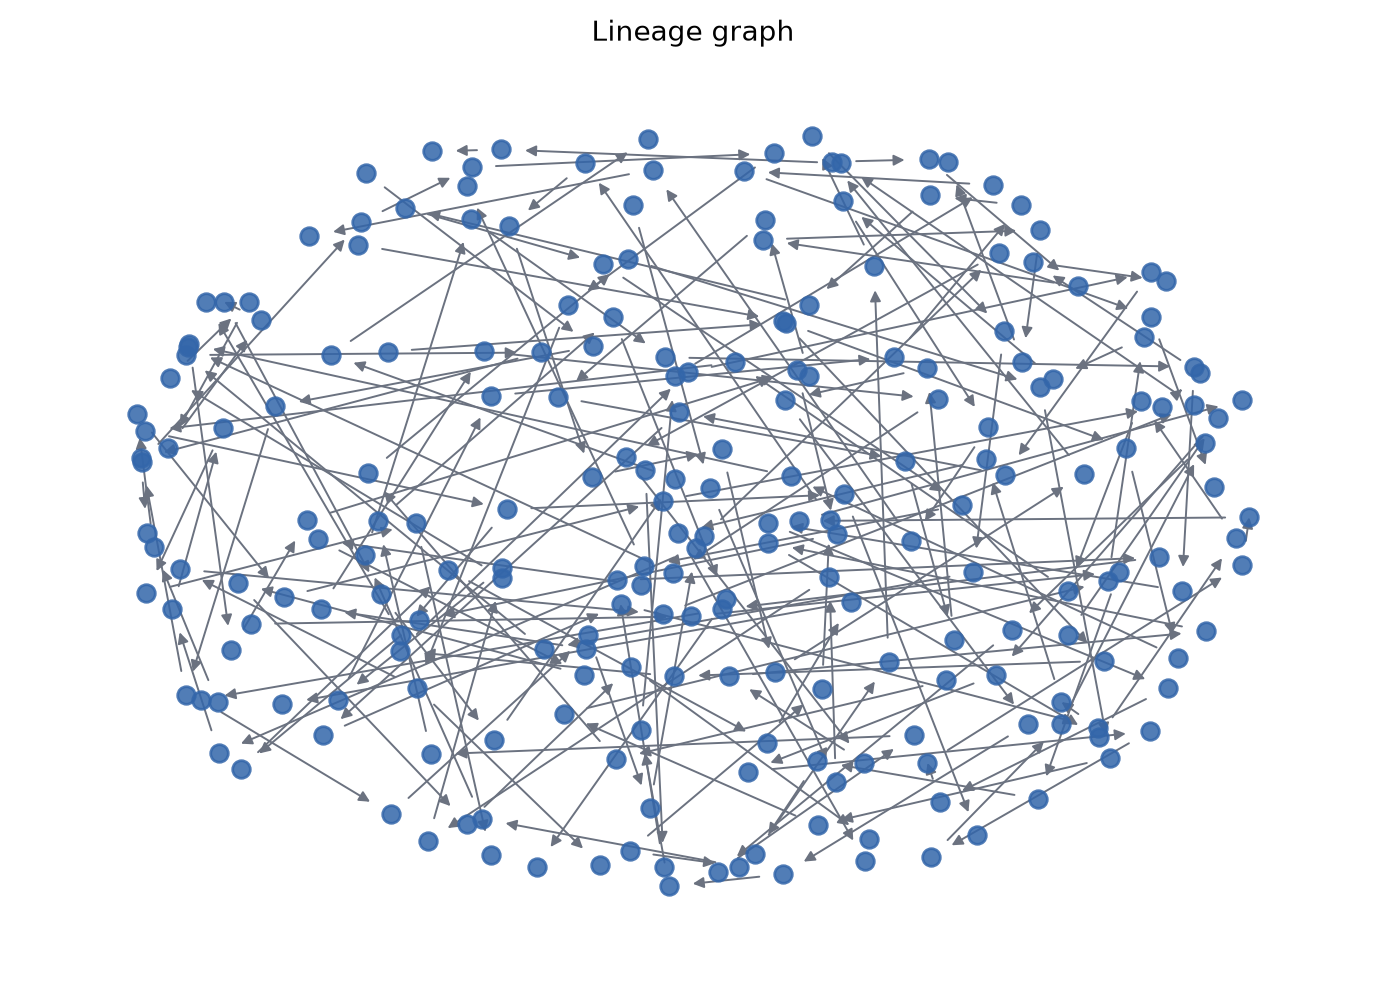
\includegraphics[width=\linewidth]{../figures/lineage_graph.png}
  \caption{Example lineage graph rendered from exported nodes and edges.}
  \label{fig:lineage}
\end{figure}

\section{Qualitative Evaluation}
We evaluate the system qualitatively on synthetic fluorescent volumes and on zebrafish-style anisotropic data when available.
Figure~\ref{fig:detection} shows centroid overlays on a single slice.
Figure~\ref{fig:lineage} visualizes the reconstructed graph.
Frame-wise detection counts remain stable under default parameters, and division events appear at biologically plausible intervals in synthetic sequences with simulated mitosis.

Quantitative benchmarking against fully annotated lineages is left to datasets with dense ground truth; sparse training labels in the reference format are insufficient for complete supervised evaluation.

\section{Limitations}
Classical peak detection can under-segment dense clusters and over-detect bright artifacts near tissue boundaries.
Greedy frame-to-frame linking does not recover long occlusions without gap closing.
Division inference remains heuristic and may miss atypical mitosis geometries.
Learned detection is scaffolded but not yet bundled with pretrained weights.

\section{Future Work}
Planned extensions include marker-controlled watershed splitting, gap closing across multiple frames, integration of Cellpose or StarDist checkpoints, and benchmark metrics against dense lineage annotations when available.

\section{Conclusion}
Biohub Cell Lineage Tracker provides a transparent 3D cell tracking pipeline and an interactive environment for visual inspection and export.
By separating detection, linking, and lineage reconstruction, the system offers a practical foundation for developmental imaging studies and further methods research.

\bibliographystyle{IEEEtran}
\bibliography{references}

\end{document}
